\section{Vectorización de BFS}

La paralelización de este algoritmo se basa fuertemente en el orden por niveles en que BFS visita los nodos. Esto es, primero visita todos los nodos que se encuentran a distancia 1 del conjunto de nodos fuente, luego visita todos los que se encuentran a distancia 2, y así sucesivamente. Formalmente, esto se expresa en que el Algoritmo \ref{algo:algoritmo5} cumple que los nodos son extraídos de la cola en orden, según la distancia al conjunto $S$. Por lo tanto, podemos clasificar por niveles a los nodos visitados, según esta distancia, de modo tal que los nodos del nivel $i$ serán aquellos que se encuentran a distancia $i$ de los nodos fuente. Los niveles se irán visitando en orden y todo nodo visitado pertenece a algún nivel. Además, notar que si el grafo a recorrer tiene $n$ nodos entonces a lo sumo hay $n$ niveles, puesto que no hay dos nodos que disten más de $n$. Por lo tanto, si conocemos los nodos que ocupan cada uno de los $n$ niveles, entonces conocemos el conjunto de nodos vistados por BFS. En la Figura \ref{fig:grafo5} se puede ver esta clasificación por niveles de los nodos de un grafo. Las aristas de trazo sólido son aquellas por las que se recorre el grafo, mientras que las de trazo punteado son aquellas por las que no se transita.

El esquema básico de las vectorizaciones que propondremos es el indicado en el Algoritmo \ref{algo:algoritmo15}.

\begin{algorithm}
	\dontprintsemicolon
	\SetKwInOut{Input}{input}
	\SetKwInOut{Output}{output}
	\Input{$G = (V, E)$ grafo\\$S$ conjunto de nodos fuente}
	\Output{$M$ conjunto de nodos visitados}
 	\BlankLine
	\Begin{
		$n = |V|$\;
		$M = S$\;
		
		\For{$i = 1$ \KwTo $n$}{
			Computar en paralelo los nodos del nivel $i$ y agregarlos a $M$\;
		}
		
		\Return $M$\;
 	}
\caption{BFS en paralelo}
\label{algo:algoritmo15}
\end{algorithm}


\begin{figure}
\begin{center}
\begin{tikzpicture}[->,>=stealth', auto, node distance=1.5cm, font=\sffamily\bfseries]
  
  \tikzstyle{nonroot}=[draw, circle, fill = black, text = black, minimum width = 6.5pt, inner sep=0pt]
  \tikzstyle{root}=[draw, circle, fill = red, text = black, minimum width = 6.5pt, inner sep=0pt]
  \node [root] (6) at (4.75, 4) [label=below:$v_{6}$] {};
  \node [root] (11) at (3.5, 0) [label=below:$v_{11}$] {};
  \node [nonroot] (14) at (4.5, 6) [label=below:$v_{14}$] {};
  \node [nonroot] (12) at (3.7, 2) [label=below:$v_{12}$] {};
  \node [nonroot] (5) at (5.5, -0.3) [label=below:$v_5$] {};
  \node [nonroot] (9) at (1.1, -0.3) [label=below:$v_9$] {};
  \node [nonroot] (1) at (1.8, 1.65) [label=below:$v_1$] {};
  \node [nonroot] (3) at (6.75, 2.75) [label=below:$v_3$] {};
  \node [nonroot] (15) at (3, 3.8) [label=below:$v_{15}$] {};
  \node [nonroot] (2) at (6, 1.5) [label=below:$v_{2}$] {};
  \node [nonroot] (16) at (4.25, -2) [label=below:$v_{16}$] {};
  \node [nonroot] (18) at (-1, 1.8) [label=below:$v_{18}$] {};
  \node [nonroot] (7) at (6.8, 5) [label=below:$v_{7}$] {};
  \node [nonroot] (10) at (8.5, 0.75) [label=below:$v_{10}$] {};
  \node [nonroot] (8) at (1.25, 3.25) [label=below:$v_{8}$] {};
  \node [nonroot] (4) at (-1.5, 4) [label=below:$v_{4}$] {};
  \node [nonroot] (13) at (0.5, 5) [label=below:$v_{13}$] {};
  \node [nonroot] (17) at (2.5, 5.5) [label=below:$v_{17}$] {};

  \path[every node/.style={font=\sffamily\small}]
  (6) edge node [] {} (14)
  (6) edge node [] {} (12)
  (11) edge node [] {} (12)
  (11) edge node [] {} (5)
  (11) edge node [] {} (9)
  (11) edge node [] {} (1)
  (12) edge node [] {} (3)
  (12) edge node [] {} (15)
  (12) edge node [] {} (5)
  (5) edge node [] {} (2)
  (5) edge node [] {} (16)
  (9) edge node [] {} (18)
  (1) edge node [] {} (18)
  (3) edge node [] {} (6)
  (3) edge node [] {} (7)
  (3) edge node [] {} (10)
  (15) edge node [] {} (8)
  (2) edge node [] {} (10)
  (18) edge node [] {} (8)
  (18) edge node [] {} (4)
  (18) edge node [] {} (13)
  (7) edge node [] {} (14)
  (8) edge node [] {} (17)
  (13) edge node [] {} (17);
\end{tikzpicture}
\end{center}

\begin{center}
\begin{tikzpicture}[->,>=stealth', auto, node distance=1.5cm, font=\sffamily\bfseries]
  
  \tikzstyle{nonroot}=[draw, circle, fill = black, text = black, minimum width = 6.5pt, inner sep=0pt]
  \tikzstyle{root}=[draw, circle, fill = red, text = black, minimum width = 6.5pt, inner sep=0pt]

  \node [root] (1) at (0, 0) [label=$v_6$] {};
  \node [root] (2) at (6, 0) [label=$v_{11}$] {};
  \node [nonroot] (3) at (-0.75, -1.25) [label=$v_{14}$] {};
  \node [nonroot] (4) at (0.75, -1.25) [label=$v_{12}$] {};
  \node [nonroot] (5) at (4.5, -1.25) [label=$v_5$] {};
  \node [nonroot] (6) at (6, -1.25) [label=$v_9$] {};
  \node [nonroot] (7) at (7.5, -1.25) [label=$v_1$] {};
  \node [nonroot] (8) at (0, -2.5) [label=$v_3$] {};
  \node [nonroot] (9) at (1.5, -2.5) [label=$v_{15}$] {};
  \node [nonroot] (10) at (3.75, -2.5) [label=$v_{2}$] {};
  \node [nonroot] (11) at (5.25, -2.5) [label=$v_{16}$] {};
  \node [nonroot] (12) at (6, -2.5) [label=$v_{18}$] {};
  \node [nonroot] (13) at (-0.75, -3.75) [label=$v_{7}$] {};
  \node [nonroot] (14) at (0.75, -3.75) [label=$v_{10}$] {};
  \node [nonroot] (15) at (5, -3.75) [label=$v_{8}$] {};
  \node [nonroot] (16) at (6, -3.75) [label=$v_{4}$] {};
  \node [nonroot] (17) at (7, -3.75) [label=$v_{13}$] {};
  \node [nonroot] (18) at (7, -5) [label=$v_{17}$] {};

  \path[densely dotted]
  (13) edge [bend left] node [above] {} (3)
  (8) edge node [] {} (1)
  (2) edge [bend right] node [left] {} (4)
  (4) edge node [] {} (5)
  (9) edge node [] {} (15)
  (10) edge node [] {} (14)
  (15) edge [bend right] node [right] [] {} (18)
  (7) edge [bend left] node [below left] {} (12)
  ;

  \path[every node/.style={font=\sffamily\small}]
  (1) edge node [] {} (3)
  (1) edge node [] {} (4)
  (2) edge node [] {} (5)
  (2) edge node [] {} (6)
  (2) edge node [] {} (7)
  (4) edge node [] {} (8)
  (4) edge node [] {} (9)
  (5) edge node [] {} (10)
  (5) edge node [] {} (11)
  (6) edge node [] {} (12)
  (8) edge node [] {} (13)
  (8) edge node [] {} (14)
  (12) edge node [] {} (15)
  (12) edge node [] {} (16)
  (12) edge node [] {} (17)
  (17) edge node [] {} (18);
\end{tikzpicture}
\end{center}
\caption{Clasificación de los nodos de un grafo por niveles}
\label{fig:grafo5}
\end{figure}

\subsection{Algoritmo $\mathcal{O}(n^3)$}

Dado el grafo $G$, enumeremos sus nodos de 1 a $n$. Supongamos que está representado mediante una matriz de adyacencia, que llamamos $A_G$. Para cada $k = 1, \cdots, n$, supongamos que $fil_k(A_G)$ es un arreglo de $n$ elementos, que representa la fila $k$ de la matriz $A_G$. Notemos que $fil_k(A_G)$ indica los nodos en los que incide el nodo $k$.

Supongamos que deseamos calcular los nodos del nivel $i \geq 1$. El resultado clave es el siguiente.

\begin{prop}
\label{prop:prop1}
Los nodos del nivel $i$ son exactamente aquellos que son incididos por algún nodo del nivel $i - 1$ pero que aún no han sido visitados.
\begin{proof}
Sea $v$ un nodo perteneciente al nivel $i$, entonces $v$ se encuentra a distancia $i$ del conjunto $S$ de nodos fuente. Consideremos un camino $\langle v_0, \cdots, v_i = v \rangle$ que realice esa distancia. Dicho camino comienza en un nodo fuente y termina en $v$. El nodo $v_{i - 1}$ necesariamente dista $i - 1$ del conjunto $S$, pues $d(S, v_{i - 1}) \leq i - 1$ y no puede distar menos que esto porque de lo contrario tendríamos $d(S, v) < i$. Por lo tanto, $d(S, v_{i - 1}) = i - 1$ con lo cual $v_{i - 1}$ es un nodo del nivel $i - 1$ que incide en $v$.

Recíprocamente, si un nodo $v$ aún no visitado es incidido por un nodo del nivel $i - 1$, entonces $d(S, v) > i - 1$, porque de lo contrario ya habría sido visitado en algún nivel inferior a $i$, y además $d(S, v) \leq i$ porque existe un camino de $S$ a $v$ que usa $i$ aristas, que es el camino que pasa por el nodo incidente del nivel $i - 1$. Entonces $d(S, v) = i$, con lo cual $v$ se encuentra en el nivel $i$.
\end{proof}
\end{prop}

Antes de usar esta proposición necesitamos introducir algunos conceptos y operaciones involucradas en el algoritmo.

\begin{defi}
Dado un arreglo $X[1\twodots n]$, decimos que $X$ es un arreglo binario de $n$ elementos si para cada $k = 1, \cdots, n$, $X[k]$ vale 0 o 1.
\end{defi}

\begin{defi}
Definimos la operación binaria $\textsf{AND}$, cerrada en los arreglos binarios, del siguiente modo. Dados $X, Y$ arreglos binarios de $n$ elementos, $X \textsf{ AND } Y$ es un arreglo binario de $n$ elementos tal que para cada $k = 1, \cdots, n$,

\[(X\textsf{ AND }Y)[k] = X[k] \textsf{ and } Y[k] 
\]

donde el operador $\textsf{and}$ es la conjunción lógica clásica. Análogamente se definen $\textsf{OR}$ y $\textsf{NOT}$ como

\[(X\textsf{ OR }Y)[k] = X[k] \textsf{ or } Y[k] 
\]

\[(\textsf{NOT }X)[k] = \textsf{not } X[k] 
\]

donde el operador $\textsf{or}$ es la disyunción lógica y $\textsf{not}$ es la negación lógica.\\[0.25cm]
\end{defi}

Definimos $X$ como el arreglo de $n$ elementos que contiene los nodos del nivel $i - 1$, es decir,

\[X[k] = \left\{ 
  \begin{array}{l l}
    1 & \quad \text{si el nodo } k \text{ pertenece al nivel } i - 1\\
    0 & \quad \text{si no}
  \end{array} \right.
\]

Llamemos $M$ al arreglo binario que indica los elementos marcados hasta el momento. Si $X[k] = 1$ entonces los nodos del nivel $i$ en los que incide el nodo $k$ son exactamente $fil_k(A_G) \textsf{ AND } (\textsf{NOT }M)$. Definamos un arreglo $I_k$ que indica si el elemento $X[k]$ se encuentra en el nivel $i - 1$, esto es, $I_k = \langle X[k], X[k], \cdots, X[k] \rangle$. Entonces $fil_k(A_G) \textsf{ AND }(\textsf{NOT } M) \textsf{ AND } I_k$ contiene ceros si el nodo $k$ no se encuentra en el nivel $i - 1$ y contiene los nodos del nivel $i$ en los que incide $k$ en caso de que $k$ pertenezca al nivel $i - 1$.

Definamos $Y$ como el arreglo binario que indica los nodos pertenecientes al nivel $i$.

\begin{prop}
\label{prop:prop2}
$Y = \textsf{ OR}_{1 \leq k \leq n} (fil_k(A_G) \textsf{ AND } (\textsf{NOT }M) \textsf{ AND } I_k)$.

\begin{proof}
Se sigue de la Proposicion \ref{prop:prop1}, que dice que los nodos del nivel $i$ son aquellos incididos por algún nodo del nivel $i - 1$ pero que aún no han sido visitados.
\end{proof}
\end{prop}

Esta proposición nos da una forma de computar los nodos de cada nivel, dando lugar al Algoritmo \ref{algo:algoritmo16}. 

\begin{algorithm}
	\dontprintsemicolon
	\SetKwInOut{Input}{input}
	\SetKwInOut{Output}{output}
	\Input{$G = (V, E)$ grafo\\$S$ conjunto de nodos fuente}
	\Output{$M$ conjunto de nodos visitados}
 	\BlankLine
	\Begin{
		$n = |V|$\;
		Sean $M, X, Y$ arreglos de $n$ elementos\;
		\For{$i = 1$ \KwTo $n$}{
			$M[i] = S[i]$\;
			$X[i] = S[i]$\;
		}
		\For{$i = 1$ \KwTo $n$}{
			Setear cada posición de $Y$ en 0\;
			\For{$k = 1$ \KwTo $n$}{
				Sea $I$ un arreglo de $n$ elementos\;
				Inicializar cada posición de $I$ en $X[k]$\;
				$Y = Y \textsf{ OR } (fil_k(A_G) \textsf{ AND } (\textsf{NOT }M) \textsf{ AND } I)$\;
			}
			$M = M \textsf{ OR } Y$\;
			$X = Y$\;
		}
		
		\Return $M$\;
 	}
\caption{Cómputo utilizando la Proposición \ref{prop:prop2}}
\label{algo:algoritmo16}
\end{algorithm}

En la Figura \ref{fig:arreglos_niveles} se pueden ver cada uno de los niveles del grafo de la Figura \ref{fig:grafo5} representado mediante arreglos de bits. Esto ilustra cómo es posible pensar un recorrido BFS en términos de arreglos de bits. La figura incluye sólo las aristas transitadas por la búsqueda.

\begin{figure}[h]
\centering
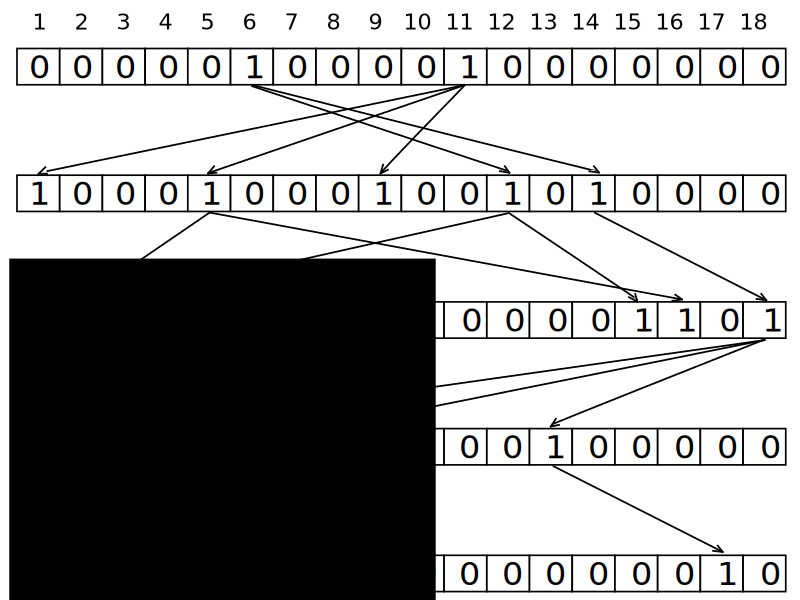
\includegraphics[scale=0.3]{imagenes/bfs.png}
\caption{Niveles representados por arreglos de bits}
\label{fig:arreglos_niveles}
\end{figure}

Notemos que si bien en cada iteración del ciclo 10-14 computamos estrictamente los nodos del nivel $i$ (es decir, $Y$ nunca contiene nodos que no pertenezcan al nivel que se está calculando) podemos relajar un poco esta condición ya que, para llegar al resultado, lo único que nos necesitamos saber es si cada nodo del grafo pertenece a algún nivel, y no nos interesa saber a cuál. Esto es, en lugar de pedir que $Y$ contenga sólo los nodos del nivel $i$, pedimos que contenga los nodos de los niveles $0, \cdots, i$. Pero notemos que esta condición ya es cumplida por el arreglo $M$ a lo largo del ciclo. Esta situación es un indicio de que podemos prescindir del arreglo $Y$, utilizando directamente $M$. Lo que falta es ver cómo hacemos crecer el conjunto $M$ a lo largo de las iteraciones. En otras palabras, teniendo todos los nodos de los niveles $0, \cdots, i - 1$, ¿cómo agregamos los nodos del nivel $i$?. La respuesta es sencilla y está sintetizada en la siguiente proposición.

\begin{prop}
\label{prop:prop3}
Sea $M$ el conjunto de nodos de los niveles $1, \cdots, i - 1$. Entonces los nodos del nivel $i$ son exactamente aquellos que no están en $M$ y que son incididos por algún nodo de $M$.

\begin{proof}
Si $v$ es un nodo del nivel $i$, entonces no pertenece a $M$ por definición, y además es incidido por algún nodo de $M$ por la Proposición \ref{prop:prop1}.

Recíprocamente, sea $v$ un nodo tal que $v \notin M$ y es incidido por algún nodo de $M$. Como $v \notin M$ entonces se encuentra en un nivel mayor o igual que $i$, es decir, $d(S, v) \geq i$. Como es incidido por algún nodo de $M$ entonces existe un camino desde un nodo fuente hacia $v$ de longitud $i$ o menos, con lo cual $d(S, v) \leq i$. Entonces $d(S, v) = i$ y por ende $v$ se encuentra en el nivel $i$.
\end{proof}
\end{prop}

Por lo tanto, para agregar a $M$ los nodos del nivel $i$ basta agregar los nodos incididos por aquellos contenidos en $M$, pero que no estén en $M$. Dado que un conjunto no contiene elementos repetidos, agregar elementos que ya estén en $M$ no hace daño, con lo cual podemos agregar nodos a $M$ sin preocuparnos por la condición de la no pertenencia.

Pero podemos ir todavía más allá y admitir que $M$ tenga, además de todos los nodos de los niveles $0, \cdots, i$, algunos nodos de niveles superiores a $i$. Esto queda plasmado en el Algoritmo \ref{algo:algoritmo17} que, a lo largo del ciclo 8-12, modifica el arreglo $M$ al mismo tiempo que lo utiliza para calcular nuevos valores, pues el arreglo $I$ se construye a partir de elementos de $M$ que posiblemente hayan sido modificados en la ejecución actual del ciclo 7-13.

\begin{algorithm}
	\dontprintsemicolon
	\SetKwInOut{Input}{input}
	\SetKwInOut{Output}{output}
	\Input{$G = (V, E)$ grafo\\$S$ conjunto de nodos fuente}
	\Output{$M$ conjunto de nodos visitados}
 	\BlankLine
	\Begin{
		$n = |V|$\;
		Sea $M$ un arreglo de $n$ elementos\;
		\For{$i = 1$ \KwTo $n$}{
			$M[i] = S[i]$\;
		}
		\For{$i = 1$ \KwTo $n$}{
			\For{$k = 1$ \KwTo $n$}{
				Sea $I$ un arreglo de $n$ elementos\;
				Inicializar cada posición de $I$ en $M[k]$\;
				$M = M \textsf{ OR } (fil_k(A_G) \textsf{ AND } I)$\;
			}
		}
		
		\Return $M$\;
 	}
\caption{$\textsc{Vectorized-BFS-No-Branching}$}
\label{algo:algoritmo17}
\end{algorithm}

Para probar que el algoritmo sigue siendo correcto, veamos que el siguiente invariante se mantiene:

\begin{center}
\emph{
	Al principio de cada iteración del ciclo 8-12, el arreglo $M$ sólo contiene (como conjunto) elementos visitados por BFS y, particularmente, contiene todos los nodos de los niveles $0, \cdots, i - 1$.
}
\end{center}

Debemos ver que el invariante es cierto al ingresar al ciclo y que se mantiene de una iteración a la siguiente.

\begin{itemize}
\item \textbf{Inicialización. } Al ingresar al ciclo, $M$ contiene únicamente nodos fuente, que son visitados por BFS. En este punto vale $i = 1$, y $M$ contiene todos los nodos del nivel 0. Entonces vale el invariante.

\item \textbf{Mantenimiento. } Supongamos que vale el invariante al principio de una iteración. Entonces $M$ sólo contiene elementos visitados por BFS y, en particular, todos los nodos de los niveles $0, \cdots, i - 1$. Por la línea 11, sólo se agregan a $M$ elementos incididos por nodos de ese mismo conjunto. Entonces todos los nodos agregados a $M$ serán alcanzables desde los nodos que contenía $M$ al ingresar al ciclo 8-12. Además, al ingresar al ciclo 8-12, $M$ sólo contiene, por la validez del invariante, elementos visitados por BFS. Luego, el ciclo 8-12 sólo agrega a $M$ elementos alcanzables desde nodos visitados por BFS, y por ende los nodos agregados también son visitados por BFS.

Veamos ahora que al concluir el ciclo 8-12, $M$ contiene todos los nodos de los niveles 0 a $i$. Es claro que contendrá todos los nodos de los niveles $0, \cdots, i - 1$, por la validez del invariante y porque el ciclo 8-12 no quita elementos de $M$. Además agrega todos los nodos del nivel $i$, porque $k$ itera sobre los nodos del nivel $i - 1$ (entre muchos otros) y agrega todos los nodos en los que inciden. Por la Proposición \ref{prop:prop1}, el ciclo 8-12 agrega, en particular, todos los nodos del nivel $i$.

Al comenzar una nueva iteración del ciclo 7-13 se incrementa el valor de $i$ y se reestablece el invariante. 

\item \textbf{Finalización. } Al finalizar el ciclo vale que $i = n + 1$ y por lo tanto se tiene que $M$ contiene sólo nodos visitados por BFS y todo nodo perteneciente a un nivel entre 0 y $n$ está en $M$. Esto es, $M$ contiene exactamente los nodos que visita BFS.
\end{itemize}

Entonces $\textsc{Vectorized-BFS-No-Branching}$ es correcto. Observemos que la principal ventaja que tiene frente al Algoritmo \ref{algo:algoritmo16} es su menor requerimiento espacial ya que no necesita de los arreglos auxiliares $X$ e $Y$. Más aún, si realizamos los cómputos directamente sobre el arreglo de entrada $S$ podemos hacer que el algoritmo sea in-place.

El Algoritmo \ref{algo:algoritmo17} es una versión vectorizada de BFS ya que las operaciones $\textsf{AND}$, $\textsf{OR}$ y $\textsf{NOT}$ se pueden realizar en paralelo utilizando el modelo SIMD. Al emplear esta técnica de paralelización se busca exprimir al máximo la performance del procesador por lo que se evita la introducción de instrucciones de decisión, que perjudican la capacidad de branching prediction. El nombre de $\textsc{Vectorized-BFS-No-Branching}$ se debe, justamente, a que nunca utiliza una estructura de decisión.

\subsubsection{Complejidad}
La complejidad del Algoritmo \ref{algo:algoritmo17} es claramente $\mathcal{O}(n^3)$ pues el costo está dominado por las líneas 7-13, conformadas por dos ciclos anidados más las operaciones lógicas a nivel de arreglos, que son $\mathcal{O}(n)$.

\subsubsection{Implementación}
Implementamos el Algoritmo \ref{algo:algoritmo17} en assembler de un procesador Intel® Core™ i5-3470, utilizando la tecnología SSE de Intel para la vectorización. Dicha implementación es escencialmente igual al algoritmo exhibido, ya que las operaciones \textsf{AND} y \textsf{OR} son computadas por las funciones \texttt{PAND} y \texttt{POR} brindadas por SSE. La diferencia yace en la forma en que realizamos tales operaciones lógicas sobre arreglos. Mientras que en el algoritmo estamos considerando que dichas operaciones se realizan elemento a elemento, la implementación las ejecuta en forma vectorizada. Más precisamente, para realizar la instrucción de la línea 11 utilizamos registros XMM de 16B, levantando en ellos bloques consecutivos de los arreglos $M$, $fil_k(A_G)$ e $I$.

Dado que todos los arreglos son binarios, podemos dotarlos de una representación compacta en forma de arreglos de bits (bits dispuestos en forma contigua en memoria). Esta opción resulta adecuada, además, debido al tipo de operaciones SSE que realizamos. En general, dado que las funciones vectorizadas operan sobre bloques de bytes de un registro, no es posible procesar en paralelo bloques con una granularidad más pequeña que 1B. La particularidad de las funciones \texttt{PAND} y \texttt{POR} es que su efecto es el mismo en cualquier bloque de cualquier tamaño del registro involucrado, pues operan sobre cada uno de los bits independientemente.

Bajo esta representación podemos paralelizar a nivel de bits y por lo tanto operar de a $16 \times 8 = 128$ elementos de los arreglos en simultaneo. Teniendo en cuenta esto, hemos requerido que el arreglo $S$ de entrada, así como cada fila de la matriz de adyacencia de $G$, tengan una longitud múltiplo de 16B. Pese a que es posible relajar esta precondición (podemos pedir solamente que la longitud sea mayor o igual a 16B), optamos por mantenerla ya que hace más sencillo el código y no agrega costo espacial ni temporal. El único requerimiento adicional sobre el input es el almacenamiento en memoria por filas de la matriz de adyacencia $A_G$, debido a que cada fila de dicha matriz es leída de a bloques consecutivos.

\subsection{Algoritmo $\mathcal{O}(n^2)$}

El Algoritmo \ref{algo:algoritmo16} desperdicia mucho tiempo ejecutando iteraciones del ciclo 10-14, para los nodos $k$ que no se encuentran en el nivel $i - 1$ (aquellos para los que $X[k] = 0$). En esos casos, el arreglo $I$ no contiene más que ceros y no se modifica el contenido del arreglo $Y$. Vamos a sacrificar un poco de capacidad de predicción de saltos introduciendo una guarda que verifique esto.

\begin{algorithm}
	\dontprintsemicolon
	\SetKwInOut{Input}{input}
	\SetKwInOut{Output}{output}
	\Input{$G = (V, E)$ grafo\\$S$ conjunto de nodos fuente}
	\Output{$M$ conjunto de nodos visitados}
 	\BlankLine
	\Begin{
		$n = |V|$\;
		Sean $M, X, Y$ arreglos de $n$ elementos\;
		\For{$i = 1$ \KwTo $n$}{
			$M[i] = S[i]$\;
			$X[i] = S[i]$\;
		}
		\For{$i = 1$ \KwTo $n$}{
			Setear cada posición de $Y$ en 0\;
			\For{$k = 1$ \KwTo $n$}{
				\If{$X[k] = 1$}{
					$Y = Y \textsf{ OR } (fil_k(A_G) \textsf{ AND } (\textsf{NOT }M))$\;
				}
			}
			$M = M \textsf{ OR } Y$\;
			$X = Y$\;
		}
		
		\Return $M$\;
 	}
\caption{$\textsc{Vectorized-BFS-Branching}$}
\label{algo:algoritmo18}
\end{algorithm}

El Algoritmo \ref{algo:algoritmo18} introduce esta mínima pero importante modificación. Veamos que esto reduce la complejidad temporal de la función a $\mathcal{O}(n^2)$.

\subsubsection{Complejidad}
Para cada $i = 0, \cdots, n$, llamemos $x_i$ a la cantidad de nodos en el nivel $i$. El costo del algoritmo está dominado por la ejecución de las líneas 8-17. La línea 8 es $\mathcal{O}(1)$ y se ejecuta $\mathcal{O}(n)$ veces. La línea 9 es $\mathcal{O}(n)$ y se ejecuta $\mathcal{O}(n)$ veces. La línea 10 es $\mathcal{O}(1)$ y se ejecuta $\mathcal{O}(n^2)$ veces. Las líneas 15 y 16 son $\mathcal{O}(n)$ y se ejecutan $\mathcal{O}(n)$ veces. Las líneas 11-13 cuestan $\mathcal{O}(n)$ y se ejecutan $\mathcal{O}\left(\sum_{i = 1}^{n} {x_i}\right)$ veces. Entonces el costo total del algoritmo es $\mathcal{O}\left(n^2 + n \sum_{i = 1}^{n}{x_i}\right)$. Pero $x_1 + \cdots + x_n \leq n$, pues los nodos no se repiten a lo largo de los niveles. Entonces $\sum_{i = 1}^{n} {x_i} = \mathcal{O}(n)$ y el costo del algoritmo resulta ser $\mathcal{O}(n^2)$.

\subsubsection{Implementación}

Al igual que el algoritmo anterior, la implementación resulta sencilla a partir del algoritmo. Lo único nuevo aquí es la operación \textsf{NOT}, aunque su naturaleza es la misma que la de \textsf{AND} y \textsf{OR}, y por lo tanto es igualmente fácil de traducir a instrucciones SSE.

\subsection{Experimentación}

Hemos implementado los algoritmos \textsc{BFS}, \textsc{Vectorized-BFS-No-Branching} y \textsc{Vectorized-BFS-Branching}, y se midieron los tiempos de ejecución de todos ellos, para distintos tipos de entradas.

Se esperaba que \textsc{Vectorized-BFS-No-Branching} tuviera, en cualquier escenario, la peor performance de todas, dada su complejidad $\mathcal{O}(n^3)$. La duda estaba entre \textsc{BFS}, de costo $\mathcal{O}(n + m)$, y \textsc{Vectorized-BFS-Branching}, de costo $\mathcal{O}(n^2)$. Notemos que si bien la versión vectorizada sólo depende de la cantidad de nodos del grafo, \textsc{BFS} depende de la cantidad de aristas $m$ que cuanto más denso es el grafo más se aproxima a $n(n - 1) = \mathcal{O}(n^2)$. Por este motivo, esperábamos que \textsc{BFS} tuviera un mejor desempeño para grafos ralos, pero que al incrementarse la densidad su tiempo de ejecución se equiparara al de \textsc{Vectorized-BFS-Branching}.

En los siguientes gráficos se muestran los tiempos registrados para estos dos algoritmos. Estos tiempos se midieron utilizando el registro TSC (Time Stamp Counter) del procesador. Si bien también hemos puesto a prueba la implementación de la vectorización sin branching, no los incluimos aquí ya que sus tiempos son un orden de magnitud mayor a los de los otros dos algoritmos. Hemos medido tiempos para grafos de distintos tamaños. Además, hemos variado la densidad de los grafos, utilizando un parámetro de densidad $p \in [0, 1]$. Este valor $p$ es la probabilidad de que, elegidos (en orden) dos nodos, el primero incida en el segundo. Finalmente, el tamaño del conjunto de nodos fuente tuvo, en todos los casos, cardinalidad aproximadamente $n / 100$, y tales nodos fueron tomados al azar.

\begin{figure}[H]
\centering
\input{texplots/bfs_big_010}
\caption{Densidad $p = 0.1$}
\end{figure}

\begin{figure}[H]
\centering
\input{texplots/bfs_big_025}
\caption{Densidad $p = 0.25$}
\end{figure}

\begin{figure}[H]
\centering
\input{texplots/bfs_big_050}
\caption{Densidad $p = 0.5$}
\end{figure}

\begin{figure}[H]
\centering
\input{texplots/bfs_big_075}
\caption{Densidad $p = 0.75$}
\end{figure}

\begin{figure}[H]
\centering
\input{texplots/bfs_big_100}
\caption{Densidad $p = 1$}
\end{figure}

Los resultados nos sorprendieron pues aún en los casos en los que el grafo era denso ($p \in \{0.75; 1\}$) \textsc{BFS} era más del doble de rápido que \textsc{Vectoriezd-BFS-Branching}. Puede observarse en el caso $p = 1$, que el comportamiento asintótico es el mismo, difirierdo los costos de ambas versiones en una constante. Para ver de dónde proviene esta constante, revisemos el Algoritmo \ref{algo:algoritmo18}. Las líneas 9, 15 y 16 tienen un costo $\Theta(n)$ y se ejecutan $n$ veces cada una, con lo cual cada una aporta un costo $\Theta(n^2)$ en total. Más aún, cada uno de estos factores cuadráticos tienen asociada una constante que no es pequeña, pues las operaciones involucradas son accesos a memoria principal. Recordemos que estas operaciones eran realizadas dada la necesidad de mantener separadamente los nodos calculados del nivel anterior, los nodos del nivel actual, y todos los nodos marcados. Contrariamente, \textsc{BFS} no incurre en estos costos, pues sólo necesita mantener un único conjunto de nodos marcados.